%!TEX root = ../main.tex
\chapter{CALICE Calorimeter concepts}

The CALICE Collaboration is developing and testing electromagnetic and hadronic calorimeters. These detector concepts are optimized toward a linear collider environment such as the International Linear Collider (ILC) \cite{Behnke:2013lya} or Compact Linear Collider (CLIC) \cite{2012arXiv1202.5940L} but collaboration with the Large Hadron Collider community for the High-Lumi upgrade (HL-LHC) is ongoing \cite{1748-0221-12-01-C01042}. The CALICE calorimeters are high granularity calorimeter optimized for the particle flow algorithm (Pandora PFA) providing a very detailed image of physics events.\\
Several prototypes for physics were build in the past and tested in testbeam campaigns at DESY, CERN and FNAL \cite{1748-0221-3-08-P08001, 1748-0221-5-05-P05004, 1707.07126v2, 1748-0221-10-10-P10039, 1748-0221-3-05-P05001}. Three physics prototypes of 1 m$^3$ were conceived using different active material and absorbers as well different readout schemes.\\
Nowadays, the CALICE Collaboration is still performing analysis on the data collected by these prototypes \cite{OskarCAN, YasmineCAN}. Also, the collaboration is looking forward in the integration into a full linear collider detector by designing several new technological calorimeter prototypes.\\
In this chapter, the electromagnetic and hadronic calorimeter concepts will be introduced, described and compared in details.

\section{Electromagnetic Calorimeters}

The CALICE Collaboration is developing two different electromagnetic calorimeters (ECAL) concepts. Physics prototypes whose goal was to prove the performance of such calorimeters for detailed measurements of EM showers, were first built. Now engineering prototypes are designed in order to improve the calorimeter design, the integration of the front-end electronics and the readout scheme. In the next subsections, the silicon-based SiECAL and the scintillator-based ScECAL calorimeters using both tungsten as absorber material will be described.

\subsection{SiECAL}

The SiECAL physics prototype consists of 30 active and absorber layers. The sensitive layer is made of high-resistivity silicon wafers 525 \si{\micro\meter} thick. These are divided in 6$\times$6 cm$^2$ sensors, segmented into a matrix of 1$\times$1 cm$^2$ PIN diodes operated in reversed bias. The total active area is 18$\times$18 cm$^2$ which resulted in 9720 channels. The depth of the calorimeter was 24 X$_0$ achieved by 10 layers of 0.4 X$_0$ (1.4 mm), followed by 10 layers of 0.8 X$_0$ (2.8 mm) and 10 more layers of 1.2 X$_0$ (4.2 mm) thick tungsten absorber plates. No front-end electronics was integrated into the layers but placed off-detector using analog lines. The performance of such calorimeter was tested in various beams at DESY and CERN. An energy resolution of $\frac{16.53\%}{\sqrt{E}}$ stochastic term and $1.07\%$ constant term was achieved \cite{ADLOFF2009372}.

\begin{figure}[htbp!]
  \centering
  \begin{subfigure}[t]{0.49\textwidth}
    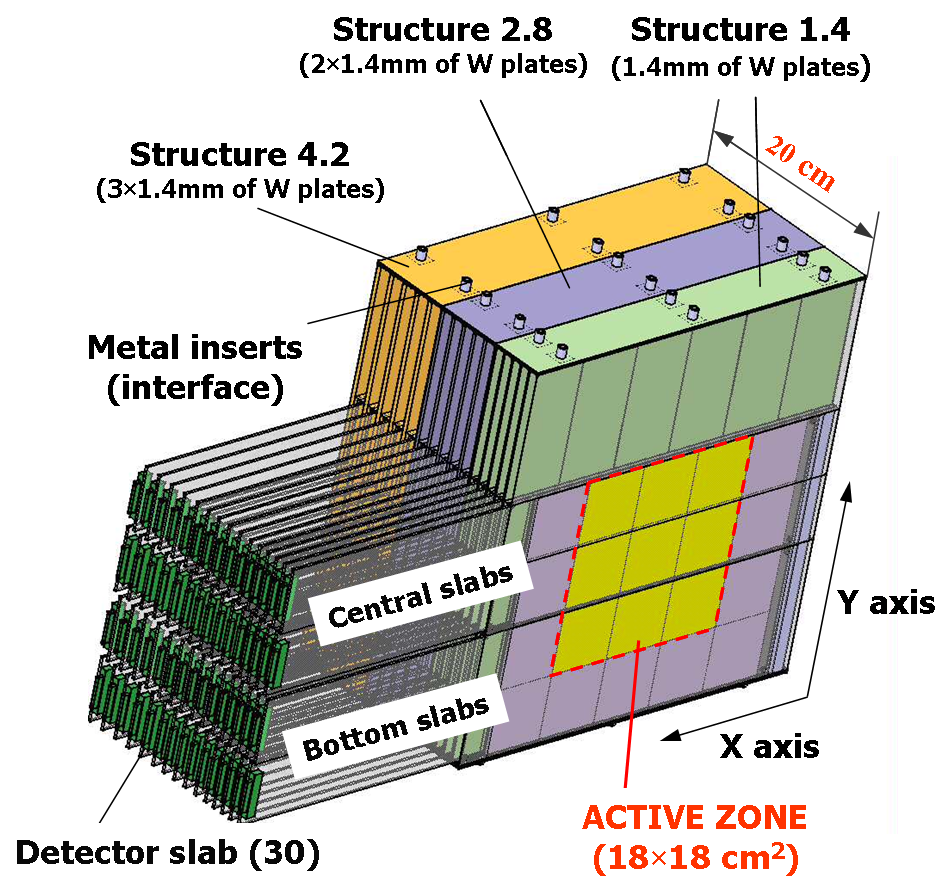
\includegraphics[width=1.\linewidth]{chap3/fig/3DProtoH.png}
    \caption{} \label{fig:SiWECALPhysics}
  \end{subfigure}
  \hfill
  \begin{subfigure}[t]{0.49\textwidth}
    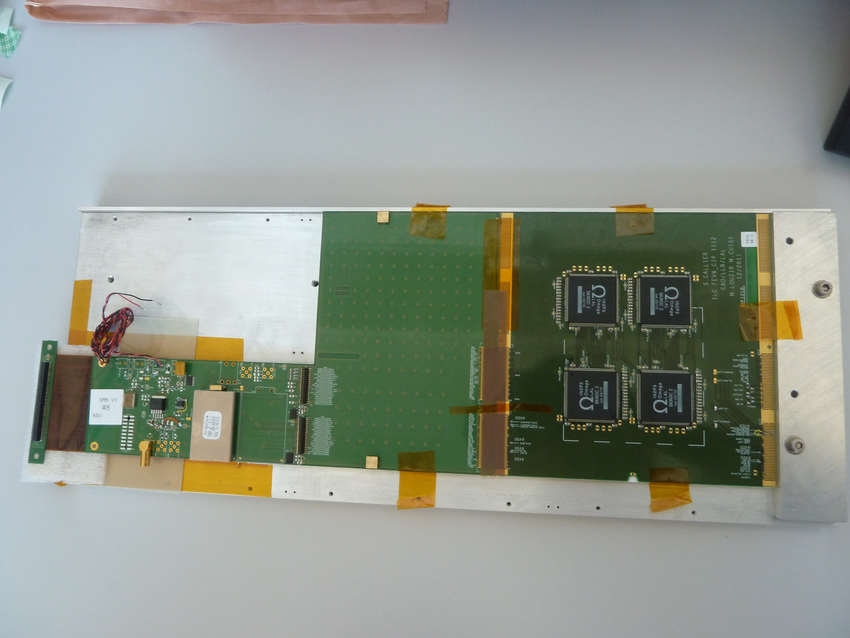
\includegraphics[width=1.\linewidth]{chap3/fig/SiW-ECAL_Techno.png}
    \caption{} \label{fig:SiWECALTechno}
  \end{subfigure}
  \caption{\subref{fig:SiWECALPhysics}) The schematics of the SiW-ECAL physics prototype. \subref{fig:SiWECALTechno}) Picture of a layer of the SiW-ECAL technological prototype.}
\end{figure}

After the validation of the calorimeter concept, a technological SiECAL prototype is being developed focusing on the integration into a full linear collider detector. To do this, modules close to the ILD design are being developed taking into account mass-production and low-power front-end electronics are integrated into the detector volume. The silicon wafers are larger and divided into 9$\times$9 cm$^2$ sensors. The PIN diode matrix is reduced to 5$\times$5 mm$^2$ pads to improve the pattern recognition of the calorimeter. New designs to the sensor are also made to minimize dead area at the sensor edge and cross-talk effects. The front-end is equipped with an ASIC, the SKIROC2 chip \cite{1748-0221-6-12-C12040}. It has 64 channels with adjustable gain charge pre-amplifier, a 12-bit ADC and digital logic. Also, it allows for auto-triggering with adjustable threshold (below 0.5 MIP) and hit time recording performed on a 12-bit TDC ramp. The SKIROC2 ASIC is designed to match the ILC beam structure (see section \ref{}) and thus allows for a power-pulsed mode where electronics are switched off between ILC bunches. This allows a very low power dissipation in the order of 25 \si{\micro\watt} per channel.

\subsection{ScECAL}
\label{subsec:ScECAL}

The ScECAL physics prototype consists of 30 layers of scintillator and tungsten carbide absorber plates 3.5 mm thick. The total calorimeter thickness is 266 mm or 21.5 X$_0$. The layers have a transverse area of 180$\times$180 mm$^2$. Each layer is composed of four rows of 18 scintillator strips of dimensions 45$\times$10$\times$3 mm$^3$ and the strips are placed orthogonally in consecutive layers. The strips have a Wavelength-shifting Fiber (WLS) inside to guide the scintillation light to a Silicon-Photomultiplier (SiPM), a MPPC from Hamamatsu. This accounts for 2160 channels to be read out. This prototype was tested in various beams, an energy resolution of $\frac{12.6\%}{\sqrt{E}}$ stochastic and 1.6\% constant term was demonstrated \cite{1707.07126v2}.

\begin{figure}[htbp!]
  \centering
  \begin{subfigure}[t]{0.49\textwidth}
    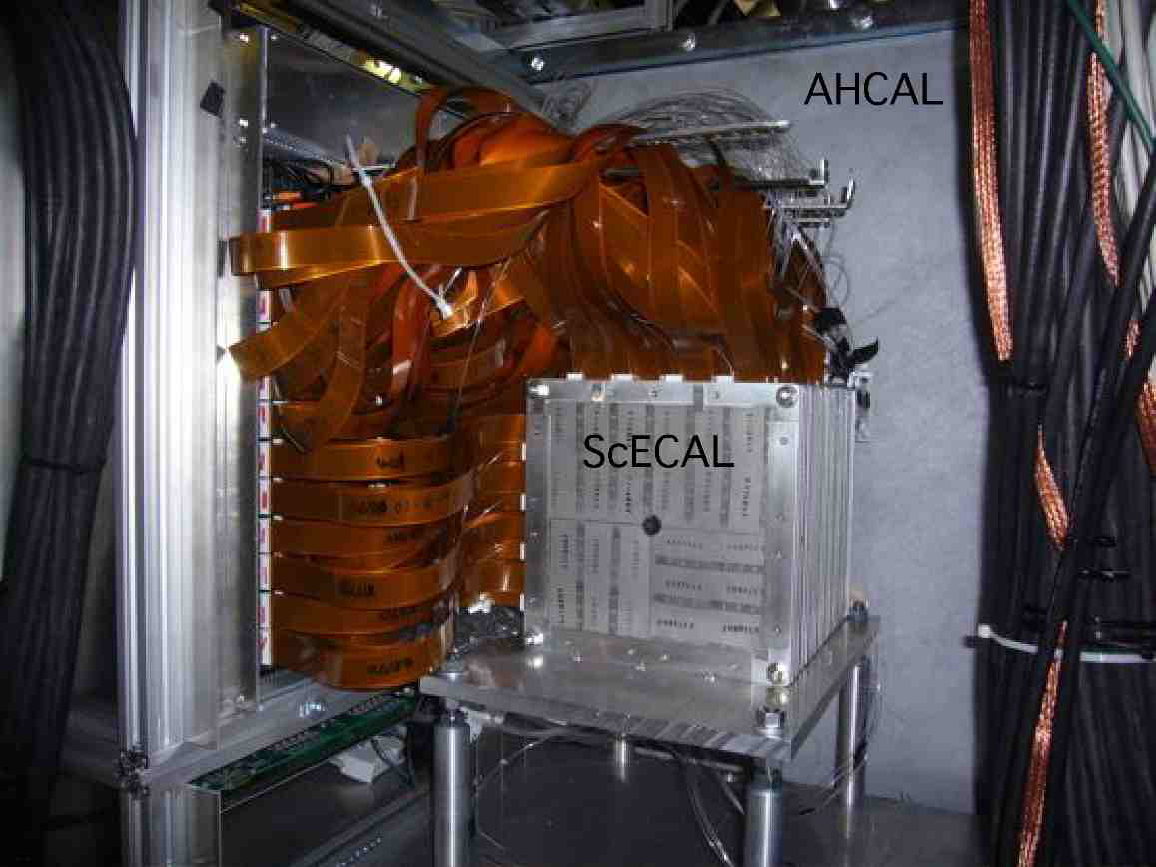
\includegraphics[width=1.\linewidth]{chap3/fig/photo_scecal2.pdf}
    \caption{} \label{fig:ScECALPhysics}
  \end{subfigure}
  \hfill
  \begin{subfigure}[t]{0.49\textwidth}
    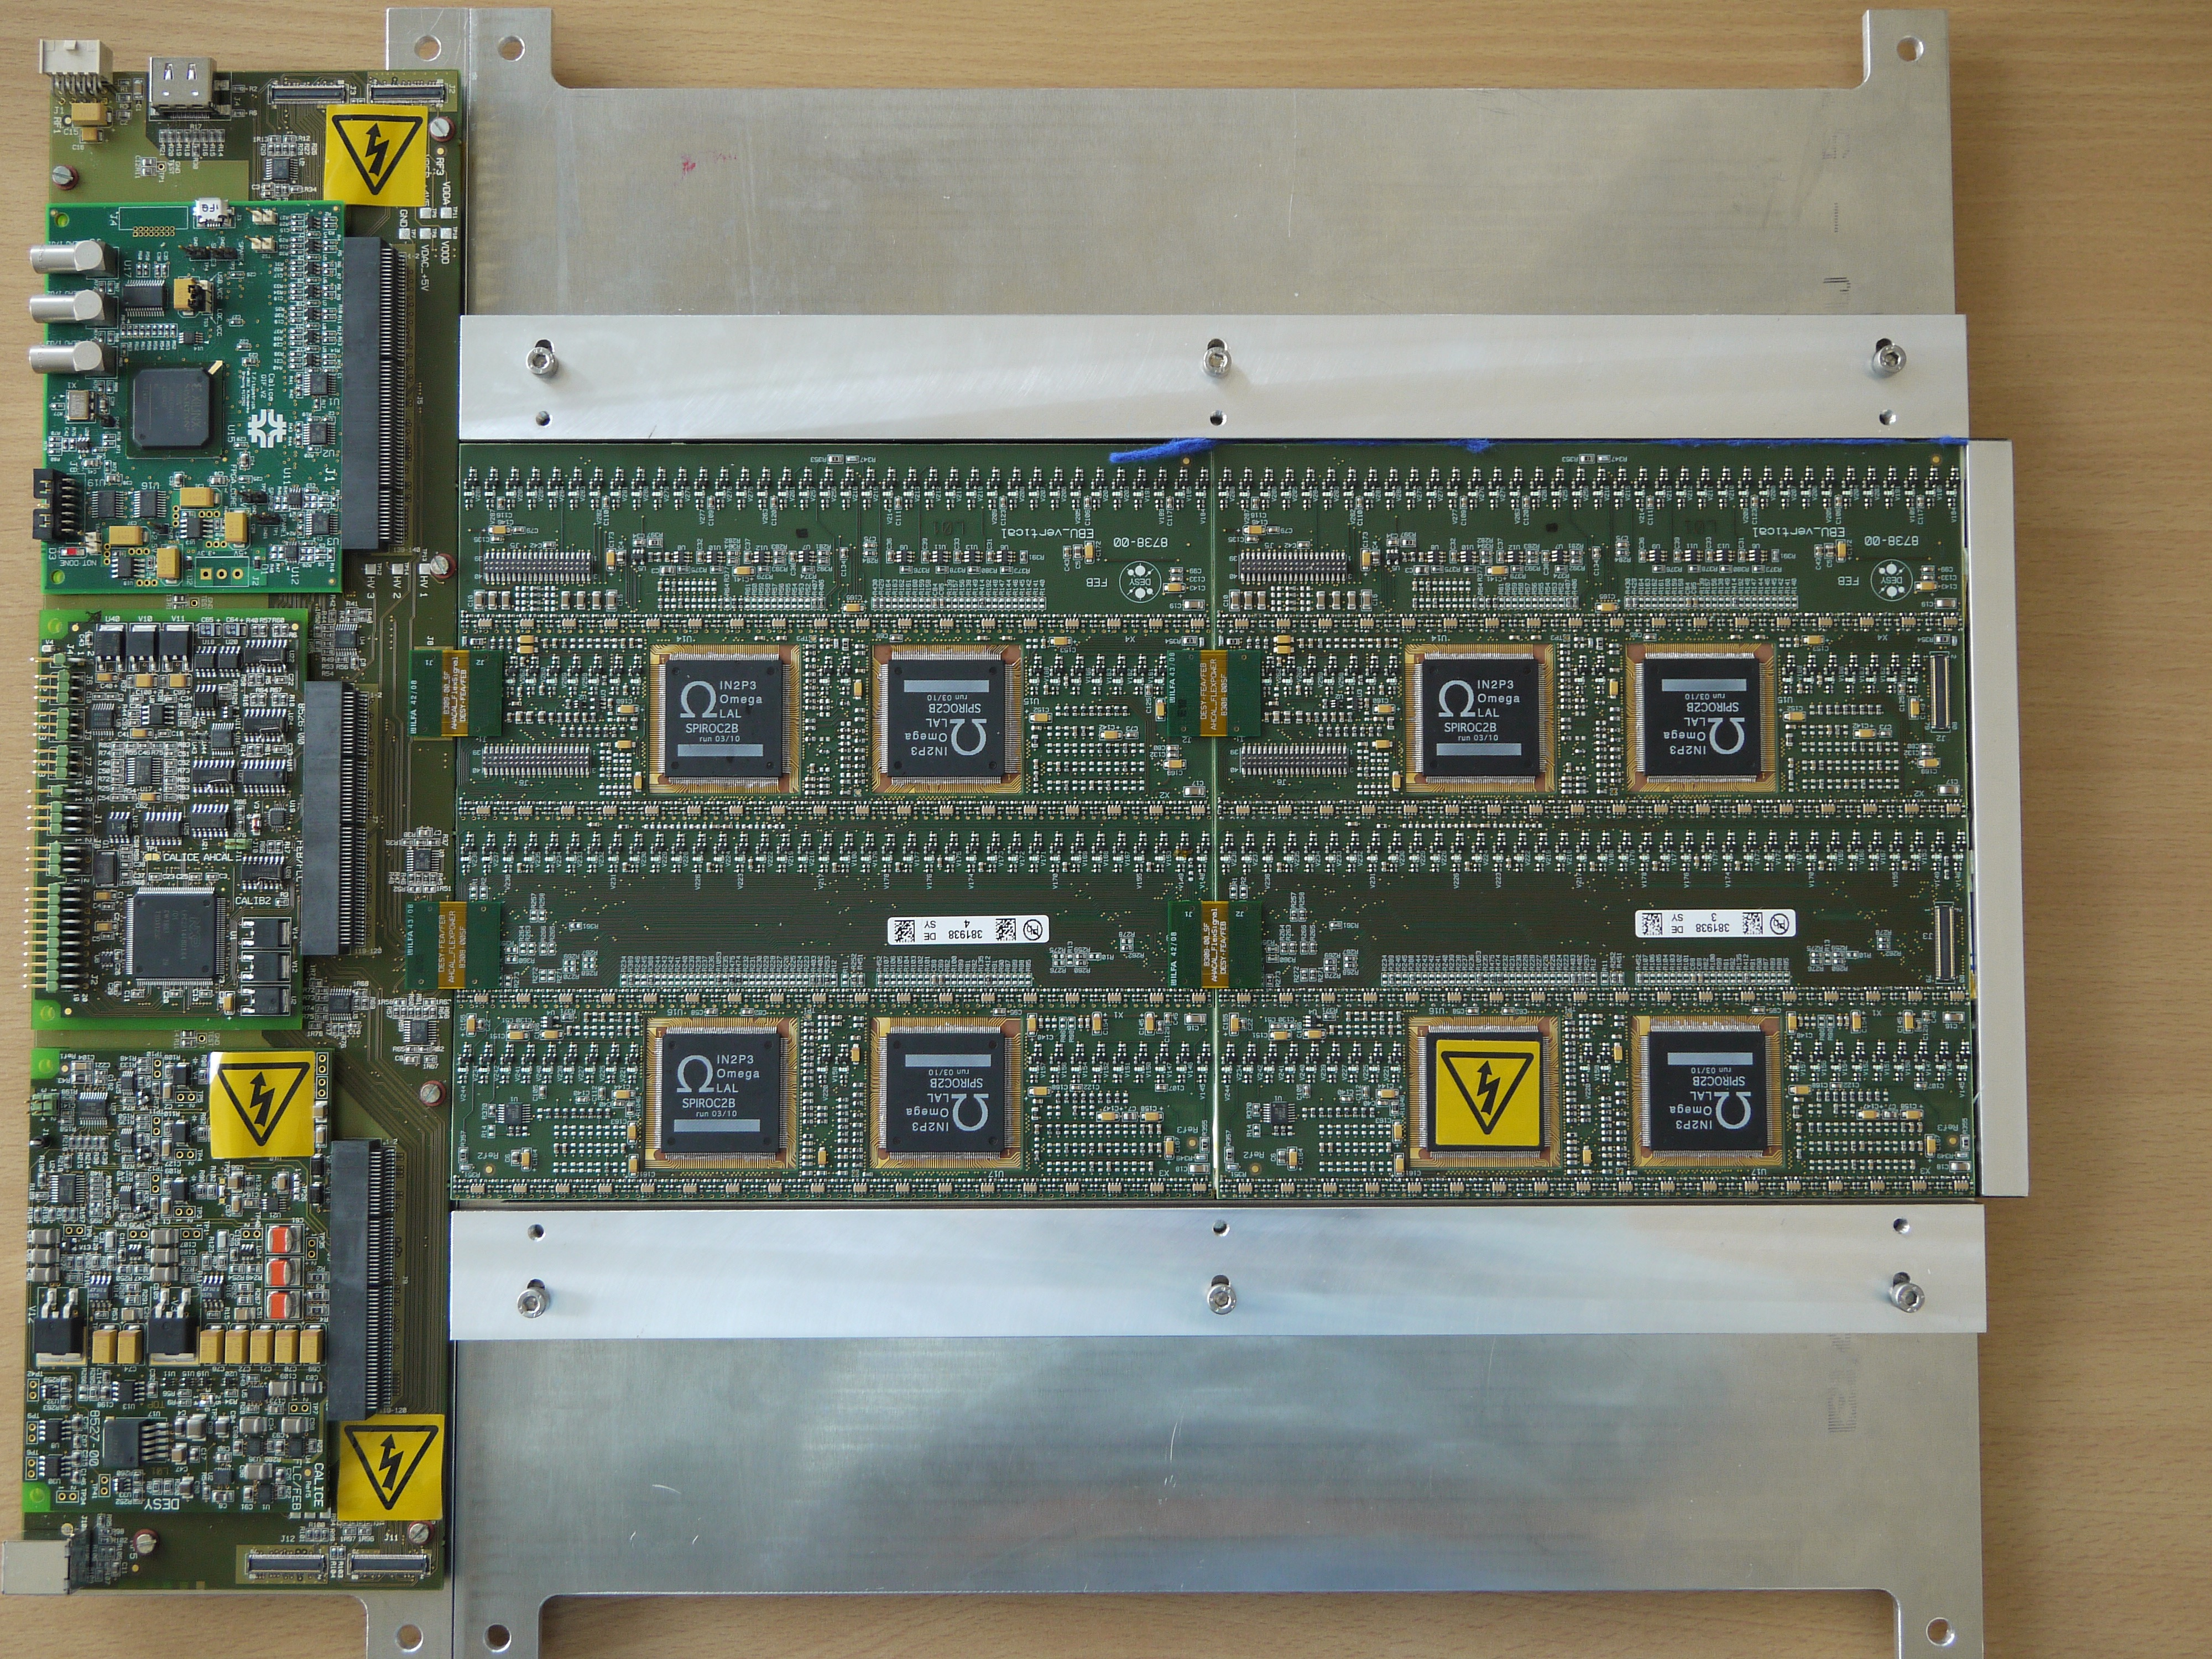
\includegraphics[width=1.\linewidth]{chap3/fig/P1060076.jpeg}
    \caption{} \label{fig:ScECALTechno}
  \end{subfigure}
  \caption{\subref{fig:ScECALPhysics}) Photo of the ScECAL physics prototype with the Fe-AHCAL at FNAL. \subref{fig:ScECALTechno}) Photo of the top side of the technological ScECAL prototype.}
\end{figure}

To look forward, a technological prototype is now developed to accommodate the front-end electronics into the layer to reduce the amount of dead material due to cabling. An ECAL Base Unit (EBU) has 144 scintillator strips of dimensions 45$\times$5$\times$2 mm$^3$. Each layer has a transverse dimension of 180$\times$180 mm$^2$. The strips don't have a WLS fiber due to improvements in SiPM technology for blue light ($\sim$ 450 nm) detection efficiency. Several designs in SiPM and scintillator strip shape are being studied to optimize light collection. In this thesis (see section \ref{}), two designs were used in testbeam at CERN, a bottom-side readout and baseline readout design. The former uses 10k pixels surface-mounted MPPC, the latter uses 1.6k pixels MPPC placed on the side of the strips. Each SiPM are read out by an ASIC, the SPIROC2B. Each layer are equipped with four SPIROC ASICs. Each channel has also an integrated LED calibration system in order to monitor the SiPM gain.

\subsubsection{SPIROC2B ASIC}

The SPIROC2B (SiPM Integrated Read-Out Chip) is a dedicated ASIC to readout and digitize the signal of 36 SiPM channels. Each channel can be tuned in bias voltage from -4.5V to 0V with a resolution of around 20-200 mV. Each channel, also, has a configurable charge pre-amplifier gain to cover a high SiPM pixel dynamic range. Each channel is equipped with a capacitor-array, called memory-cells, with a depth of 16 events. A 12-bit Wilkinson ADC is used to digitize the charge stored in the capacitor array for the amplitude and time measurement. The hit time is registered via a 12-bit TDC voltage ramp with a designed resolution of 100 ps if operated in ILC-like conditions (ramp length of 200 \si{\nano\second}), in testbeam, the theoretical time resolution is around 1.9 ns (ramp length of 4 \si{\micro\second}). The chip can be operated in power-pulsing mode where parts of the chips not needed in any given state of operation can be switched off.

\begin{figure}[htbp!]
  \centering
  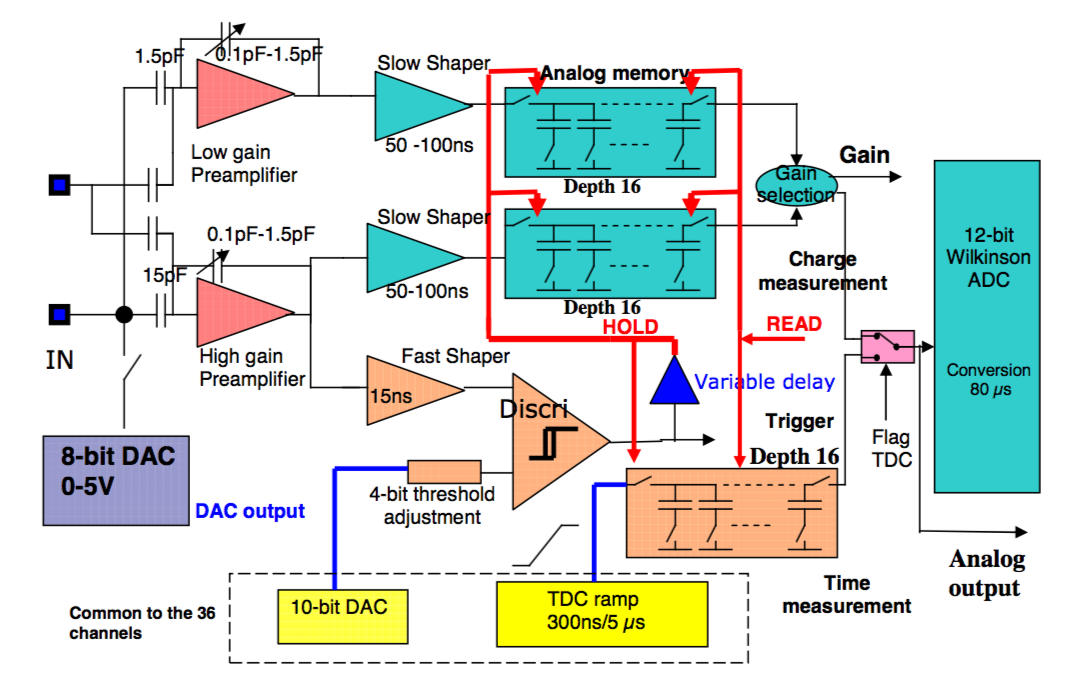
\includegraphics[width=0.7\linewidth]{chap3/fig/SPIROC2B_schematic.png}
  \caption{Schematic of the analog signal path of the SPIROC2 for a single channel \cite{SPIROC2_datasheet}.} \label{fig:SPIROC2B_sche}
\end{figure}

The chip can be operated in either external trigger mode (ET) or auto-trigger mode (AT). In external trigger, the signal of each cell is sampled synchronously to an external signal. In auto-trigger mode, the signal of each cell is compared to a configurable threshold, if the signal is above the threshold, the signal is sampled. Once the 16 memory-cells are filled, no further hits can be stored. Thus, the memory-cells are readout, digitized and the data is transferred out of the chip.

\section{Hadronic Calorimeters}

\subsection{AHCAL}
\label{subsec:SPIROC2B}

The Analog Hadron Calorimeter (AHCAL) is a sampling calorimeter using scintillator tiles has active material. The absorber structure can be either steel or tungsten but I will focus on the former one. The physics prototype consists of 38 active layers inserted in a steel structure of 1 m$^3$ with 39 absorber plates 1$\times$1 m wide and 17.4 mm thick on average. The calorimeter has a total depth of 4.28 $\lambda_{\pi}$ (5.3 $\lambda_{n}$). Active layers are consisted of a steel cassette housing 216, for the 30 first layers, or 141, for the 8 last layers, scintillator tiles connected on a PCB. The tiles are 5 mm thick and have different sizes of 3$\times$3, 6$\times$6, 12$\times$12 cm$^2$. This accounts for a total of 7608 channels. The light produced in the scintillator is guided through a WLS fiber 1 mm thick that is inserted in the tile to a SiPM. The SiPM sensitive area is 1.1$\times$1.1 mm$^2$ containing 1156 pixels which were produced by the MEPhi/PULSAR group in Russia. The performance of this prototype has been demonstrated in several beam types. For electrons, the energy resolution of the AHCAL measured is $\frac{21.7\%}{\sqrt{E}}$ stochastic and <1\% constant term \cite{CAN034}. For pions, the intrinsic energy resolution of the AHCAL has been measured to be $\frac{57.6\%}{\sqrt{E}}$ stochastic and 1.6\% constant term. This can be improved to $\frac{45\%}{\sqrt{E}}$ stochastic term by using a technique called \textit{software compensation} \cite{SoftCompNew2012}.

\begin{figure}[htbp!]
  \centering
  \begin{subfigure}[t]{0.49\textwidth}
    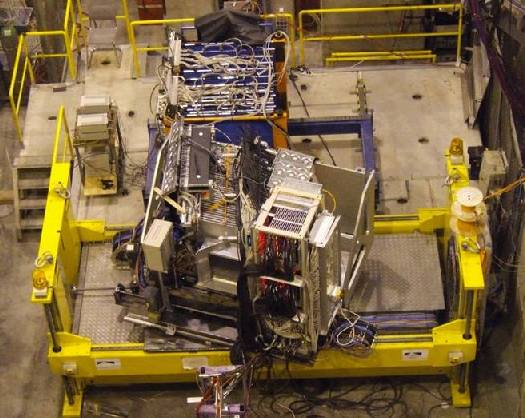
\includegraphics[width=1.\linewidth]{chap3/fig/CERN_setup.png}
    \caption{} \label{fig:AHCALPhysics}
  \end{subfigure}
  \hfill
  \begin{subfigure}[t]{0.49\textwidth}
    \includegraphics[width=1.\linewidth]{chap3/fig/moduleinside.png}
    \caption{} \label{fig:AHCALPhysics2}
  \end{subfigure}
  \caption{\subref{fig:AHCALPhysics}) Photo of the AHCAL physics prototype at CERN. \subref{fig:AHCALPhysics2}) Photo of the active layer of the AHCAL physics prototype showing the layout of the differently sized tiles.}
\end{figure}

The AHCAL engineering prototype (EPT AHCAL) is currently being studied. The goals of this prototype is to demonstrate the scalability of the AHCAL concept to a full linear collider detector. The HCAL Base Unit (HBU) is 36 cm wide PCB holding 4 SPIROC2B ASICs for a total of 144 SiPM channels coupled to a scintillator tile of 30$\times$30$\times$3 mm size to be read out. Up to 6 HBUs can be connected together to form what is called a \textit{slab}. A full AHCAL layer can be up to 3 slabs connected in parallel to a common set of readout (DIF), calibration (CALIB) and power modules (PWR). An integrated LED Calibration system can deliver LED light pulses with amplitudes to few photons up to saturation of the SiPM in order to calibrated and monitor each HBU channel. Several designs of HBU and tiles have been produced to accommodate for soldering pin or surface-mounted (SMD) type SiPMs.

\subsubsection{Current status of the EPT AHCAL}



\subsection{SDHCAL}
\subsection{DHCAL}
